\documentclass[11pt, english]{article}              
        \usepackage{geometry}
                \geometry{                          
                        a4paper,total={210mm,297mm},
                        tmargin=40.8mm,
                        bmargin=40.8mm,
                        lmargin=32.6mm,        
                        rmargin=32.6mm,                     
                }                                     
                                
	\renewcommand{\theparagraph}{\thesubsubsection.\arabic{paragraph}}

        \usepackage{titlesec}         
                \titleformat{\section}
                        {\normalfont\fontsize{18}{16}\bfseries}{\thesection}{0.5em}{}
                \titleformat{\subsection}
                        {\normalfont\fontsize{14}{16}\bfseries}{\thesubsection}{1em}{}
                \titleformat{\subsubsection} 
                        {\normalfont\fontsize{11}{16}\bfseries}{\thesubsubsection}{1em}{}
 		\titleformat{\paragraph} 
                        {\normalfont\fontsize{11}{16}\bfseries}{\theparagraph}{1em}{}

        \usepackage{longtable}                                                  
        \usepackage{multirow}                                                   
                             
        \usepackage[labelfont=bf,textfont=bf,font=small,skip=8pt]{caption}
                               
        \setlength{\parindent}{0pt}                                 
        \renewcommand{\baselinestretch}{1.25}      
        \usepackage{setspace}                             
                                                                        
        \usepackage{amsmath}                                                    
        \usepackage{amssymb}                                      
                             
        \usepackage{graphicx}                  
                               
        \usepackage{float}                                                

	\usepackage{tikz}
                                                  
\begin{document}                               
                                              
\pagenumbering{gobble}       
                       
        \title{\textsc{EC315 Topics in Microeconomics with Cross-Section Econometrics\\ Coursework Summary}}
        \author{\textsc{Lewis Britton}}
        \date{\textsc{Academic Year 2019/2020}}
        \maketitle

\newpage
                         
\pagenumbering{roman} 
                                                                           
        \renewcommand{\contentsname}{Table of Contents}
                                       
        \tableofcontents

\newpage 

\pagenumbering{arabic}

\section{Exam Summary}

	\subsection{Cost-Benefit Analysis Summary}

	\begin{enumerate}
	\setlength\itemsep{0cm}
		\item Purpose
		\item Alternatives
		\item Who
		\item C/B Impacts
		\item Lifetime Impacts
		\item Monetize:
		\begin{itemize}
			\item \textit{Social Cost}: harm done to living organisms
			\item \textit{Revealed/Stated Preference}: willingness to pay or willingness to accept
			\begin{itemize}
				\item Revealed: shown in behaviour
				\item Stated: questionnaires etc.
			\end{itemize}
			\item \textit{Time}:
			\begin{itemize}
				\item Work vs leisure using wage rate 
				\item Travel time; how much people are willing to trade-off
			\end{itemize}
			\item \textit{Lives}: life expectancy, pay, age, risks taken
			\item \textit{Natural Resources}: AONBs, surveys, investment, regulation
		\end{itemize}
		\item PV Discounts
		\begin{itemize}
			\item Social discount rate
			\item Intergenerational (more than 50 years)
		\end{itemize}
		\item NPV of Alternatives
		\item Sensitivity Analysis
		\item Recommend
	\end{enumerate}

	\newpage

	\subsection{Program \& Policy Evaluation Summary}

	\begin{center}Cause $\longrightarrow$ Intermediaries $\longrightarrow$ Effect\end{center}

	\begin{enumerate}
	\setlength\itemsep{0cm}
		\item Omitted Variable Bias
		\begin{itemize}
			\item Selection Bias: e.g. grades, income, area of ogigin
			\item Selection Bias 2: e.g. effort, determination, stamina
		\end{itemize}
		\item Randomized Control Trial
		\begin{itemize}
			\item Unbiased Estimator: $\bar{x}\longrightarrow\bar{\mu}$ (LLN)
			\item Unbiased Estimator: randomization
			\item $\sigma^2$: ``how much of the result is due to chance?''
			\item t-tests: causal effect; $(\bar{Y}^T-\bar{Y}^C)$
		\end{itemize}
		\item Regression
		\begin{itemize}
			\item Dummy Variables: causal variable / group
			\item Instrumental Variables: omitted variables ($\alpha$ corr. w/ $\varepsilon$)
		\end{itemize}
	\end{enumerate}

	\newpage

	\subsection{Crime \& Punishment Summary}

	\begin{enumerate}
	\setlength\itemsep{0cm}
		\item Supply: $\pi_t=\pi_i-c_i-w_i-p_i(f_i)$
		\begin{itemize}
			\item $i$ = Individual
			\item $\pi_t$ = Net Total Payoff of Crime
			\item $\pi_i$ = Expected Payoff Per Offense (Minus Costs)
			\item $c_i$ = Cost Incurred if Caught
			\item $w_i$ = Wage Rate From Non-Criminal Work
			\item $p_i$ = Probability of Aprehension \& Conviction
			\item $f_i$ = Punishment in Convicted
		\end{itemize}
		\item Normal Distribution
		\begin{itemize}
			\item Req. $\uparrow\pi,\ \uparrow\delta,\ [\bar{x}\rightarrow\mathrm{(Right\ of\ Mean)}]$
			\item Req. $\downarrow\pi,\ \downarrow\delta,\ [\leftarrow\bar{x}\mathrm{(Left\ of\ Mean)}]$
			\item Morals, enjoyment, risk, some demand for significantly higher payoffs etc. effect decision
		\end{itemize}
		\item Demand: $e_if(v_r,v_l);q$
		\begin{itemize}
			\item $e_i$ = Expenditure on Protection
			\item $v_r$ = Risk of Victimization
			\item $v_l$ = Loss of Victim
			\item $q$ = Total Crime
		\end{itemize}
		\item Derivatives
		\begin{itemize}
			\item $\frac{\partial e_i}{\partial v_i}>0$: Risk $\uparrow$, Expenditure $\uparrow$
			\item $\frac{\partial c_i}{\partial e_i}<0$: Expenditure $\uparrow$, Cost $\uparrow$
			\item $\frac{\partial\pi_i}{\partial c_i}<0$: Cost $\uparrow$, Payoff $\downarrow$
		\end{itemize}
		\item Supply / Demand
		\begin{itemize}
			\item 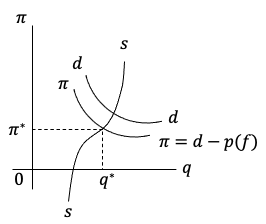
\includegraphics[width=5cm,height=4cm]{EC315-IMG/1.png}
			\item $ss$ = Supply of Crime
			\item $dd$ = Initial Demand
			\item $\pi\pi$ = Demand After Government Intervention ($T$)
			\item $MC$ of Catching Last Criminal $>$ $MB$ [$\leftarrow\pi^*,\ q^*$]
			\item $MC$ of Catching Last Criminal $<$ $MB$ [$\pi^*,\ q^*\rightarrow$]
		\end{itemize}
	\end{enumerate}

	\newpage

	\subsection{Exam Arithmetic Summary}

	\begin{enumerate}
	\setlength\itemsep{0cm}
		\item $\pi_A=x_Ap_A(x_A+x_B)-x_A$
		\item $J=\pi_A+\pi_B;\ \frac{\partial J}{\partial x_A}=\frac{\partial\pi_A}{\partial x_A}+\frac{\partial\pi_B}{\partial x_B}$
		\item Externalities: $\frac{\partial\pi_A}{\partial x_B}$
		\begin{itemize}
			\item $>0$: Positive: ``you do $\uparrow$, my $\pi$ $\uparrow$''
			\item $<0$: Negative: ``you do $\uparrow$, my $\pi$ $\downarrow$''
		\end{itemize}
		\item Strategic Nature: $\frac{\frac{\partial\pi_A}{\partial x_A}}{\partial x_B}$
		\begin{itemize}
			\item $>0$: Complements: ``you do $\uparrow$, I do $\uparrow$''
			\item $<0$: Substitutes: ``you do $\uparrow$, I do $\downarrow$''
		\end{itemize}
		\item Grim Trigger Strategy
		\begin{itemize}
			\item 40, 50, 30
			\item $\frac{40}{(1-\delta)}\ge50+\frac{30\delta}{(1-\delta)}$
			\item $40\ge50-50\delta+30\delta$
			\item $\delta\ge\frac{1}{2}$: cooperation possible
		\end{itemize}
		Tit-for-Tat Strategy
		\begin{itemize}
			\item 40, 50, 20
			\item $\frac{40}{(1-\delta)}\ge\frac{50}{(1-\delta^2)}+\frac{30\delta}{(1-\delta^2)}$
			\item $40+40\delta\ge50+20\delta$
			\item $\delta\ge\frac{1}{2}$: cooperation easy
		\end{itemize}
	\end{enumerate}

\newpage

\section{Game Theory}

	\subsection{Definitions}

	\begin{itemize}
	\setlength\itemsep{0cm}
		\item \textit{Welfare Economics}: Generalising equilibriums. Competitive markets provide an incentive for firms to produce what customers want. Markets rock in fair play.
		\begin{itemize}
			\item Theorem 1: Every competitive economy is Pareto Efficient.
			\item Theorem 2: Every Pareto Efficient allocation of resources can be achieved in competitive markets (w/ appropriate redistribution between parties).
		\end{itemize}
		\item \textit{Pareto Efficiency}: No additional person can be made better off without making someone else worse off. There should be no government intervention. Redistribution can take place meaning there is redistribution between parties within the economy rather than externally.
		\item \textit{Prisoner's Dilemma}: Pursuing your own interests leads to inefficient markets because, using the prison example, if both people choose to confess, they get full long time each. If they both lie, they get full short time. If one lies and one confesses, the one who confesses gets reduction but the liar gets full time. This is risk. Both could deny for 2 years of the other lies (gets 10 years). But then they both risk getting 8 years. If they both deny they both get the full short time (3 years). Denying is best for them both but confessing could, but only could, be best for a single one of them.
		\item \textit{Rationality}: Players will choose the option with the best payoff for themselves. But back to the Joey and Phoebe, if you are choosing the best for yourself, surely the opponent must be doing the same so can you forecast? Or will they think the same and one-up you?
		\begin{itemize}
			\item \textit{Common Knowledge of Rationality}: Where players don’t just know they possible outcomes of their decisions, they know the possible outcomes of the other’s decisions. But recall the prisoner’s dilemma.
		\end{itemize}
		\item \textit{Game Theory}: Our actions have external consequences. They effect the environment and all things around us (smoking example).
		\begin{itemize}
			\item \textit{Non-Cooperative Game}: In it for your own gain and only that.
			\item \textit{Information Game}: Everyone knows they are playing.
			\item \textit{Stage Game}: May be repeated (e.g. rearranging cost agreements).
			\item \textit{Simultaneous Game} (Type 1): When players do not know the move of the opponent and move at the same time.
			\item \textit{Sequential Game} (Type 2): When players know the move of the other player and can make their decision based on the opponent’s move. 
		\end{itemize}
		\item \textit{Imperfect/Perfect Information}: Not being able to see the others’ choice. Your outcome will always depend on their choice but your decision won’t. Or, you have information about their decision to look at as they have make it (historic forecasting).
		\item \textit{Strategic Uncertainty} (When Simultaneous): Players must base decisions on what they think the other player will play as they do not know. But then they must consider what they think the opponent’s move will be but then, the opponent will surely think they will be thinking this and so make a different move and make the same prediction about their opponent... in practice usually it comes back round to them making the first decision that you predicted they would make (Joey and Phoebe e.g.) Can lead to \textit{Strategic Payoff} where the strategic nature of their thinking pays off and they’ve well forecasted the other’s choice.
		\item \textit{Dominant Strategy}: When there is one clear winner in the strategy you use. It takes the lead the majority or all of the time when put into the matrix. This is found through \textit{Best Response Analysis} which is found by going through each option of B and selecting the best strategy for A to choose (repeat for all columns of B). Then repeating for B (for all rows of A). The double underlined is the dominant strategy.
		\item \textit{Dominated Strategy}: When the strategy a player chooses is dominated than another strategy which would make you better-off than the one you’re choosing.
		\item \textit{Nash Equilibrium}: When there is a clear equilibrium between the players' \textit{Dominant Strategies}. Means you can't \textit{Unilaterally Deviate} to become more profitable (no incentive to deviate).
		\begin{itemize}
			\item \textit{Unilateral Deviation}: When there is no dominant strategy.
			\item \textit{Mixed Strategies}: Players randomise strategies on unpredictable patterns (e.g. with muscular workouts).
			\item \textit{Pure Strategies}: When the player knows for sure what option they will choose.
		\end{itemize}
	\end{itemize}

	\newpage

	\subsection{Simultaneous Move Game}

	\begin{itemize}
	\setlength\itemsep{0cm}
		\item Sole entrant: obtains big payoff
		\item Multiple entrants: perhaps lacking market space
		\item There exists a \textit{First Mover Advantage}
	\end{itemize}

		\subsubsection{Pure \& Mixed Strategies}
	
	\begin{itemize}
	\setlength\itemsep{0cm}
		\item \textit{Chicken Game}: two players heading towards each other;
		\begin{itemize}
			\item They collide and both marginally lose out
			\item One swerves and loses out bigger (chicken)
		\end{itemize}
		\item There may be two nash equilibria
		\begin{itemize}
			\item 
				\begin{table}[h]
					\scriptsize
					\renewcommand{\arraystretch}{1.25}
				\begin{center}
				\begin{tabular}{|c|c|c|c|}
					\hline
					& \multicolumn{3}{|c|}{Player B}\\
					\hline
					\multirow{3}{*}{Player A} & & $E(q)$ & $N(1-q)$\\
					\cline{2-4}
					& $E(p)$ & $-50,100$ & $\underline{150},\underline{0}$\\
					\cline{2-4}
					& $E(1-p)$ & $\underline{0},\underline{100}$ & $0,0$\\
					\hline
				\end{tabular}
				\end{center}
				\end{table}
			\item The nash equilibria are underlined. There are two
			\item Pure strategies are shown through probability as seen by entering probabilities $p$ \& $q$ above
			\item For Player A ($EV$ = Expected Value):
				\begin{table}[h]
                                        \renewcommand{\arraystretch}{1.25}
				\begin{center}
				\begin{tabular}{l|l}
					$EV_A^E=-50q+150(1-q)$ & $EV_B^E=-100p+100(1-p)$\\
					$EV_A^N=0q+0(1-q)$ & $EV_B^N=0p+0(1-p)$\\
					$-50q+150-150q=0$ & $-100p+100(1-p)=0$\\
					\underline{$q=\frac{3}{4}$} & \underline{$p=\frac{1}{2}$}\\
				\end{tabular}
				\end{center}
				\end{table}
			\item These are the probabilities of placing in the respective quartiles:
				\begin{table}[h]
					\scriptsize
                                        \renewcommand{\arraystretch}{1.25}
                                \begin{center}      
                                \begin{tabular}{|c|c|c|}
					\hline
					& $E\frac{3}{4}$ & $N\frac{1}{4}$\\
					\hline
					$E\frac{1}{2}$ & $\frac{3}{8}$ & $\frac{1}{8}$\\
					\hline
					$N\frac{1}{2}$ & $\frac{3}{8}$ & $\frac{1}{8}$\\
					\hline
				\end{tabular}
                                \end{center} 
                                \end{table}
			\item You are trying to find the option that would make you both indifferent between choosing options
		\end{itemize}
	\end{itemize}

	\newpage

	\subsection{Sequential Move Game}
	
	\begin{itemize}
	\setlength\itemsep{0cm}
		\item Uses \textit{Backward Induction}
		\begin{itemize}
			\item Games are analysed from the end through to start
		\end{itemize}
		\item Transforms \textit{Normal Form} to \textit{Extensive Form}
		\item Transforms \textit{Nash Equilibrium} to \textit{Sub-Game Nash Equilibrium}
		\item Not subject to \textit{Strategic Uncertainty} (imperfect information)
		\begin{itemize}
			\item Can observe moments
			\item Hence, \textit{Perfect Information}
			\item E.g. supermarket price setting
		\end{itemize}
		\item If the first or last mover has a \textit{Dominant Strategy}, they'll use it
	\end{itemize}

		\subsubsection{Game Tree}

	\tikzstyle{level 1}=[level distance=2cm, sibling distance=8cm]
        \tikzstyle{level 2}=[level distance=2cm, sibling distance=4cm]

	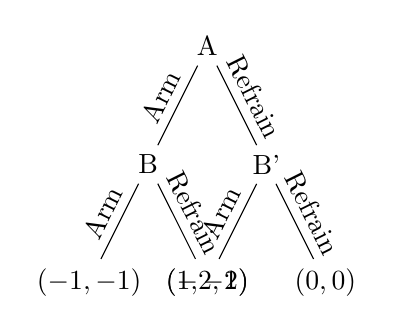
\begin{tikzpicture}[sloped]               
                \node {A}
                        child {                                
                                node {B}
                                        child {                
						node {$(-1,-1)$} 
						edge from parent
                                                        node[above] {Arm}
                                                }
                                        child {                 
						node {$(1,-2)$} 
						edge from parent
                                                        node[above] {Refrain}
                                                }
						edge from parent
                                                        node[above] {Arm}
                                }
                        child {                                
                                node {B'}
                                        child {                 
						node {$(-2,1)$} 
						edge from parent
                                                        node[above] {Arm}
                                                }
                                        child {                 
						node {$(0,0)$}
						edge from parent
                                                        node[above] {Refrain}
                                                }
						edge from parent
                                                        node[above] {Refrain}
                                };
        \end{tikzpicture}

	\begin{table}[h]
		\renewcommand{\arraystretch}{1,25}
	\begin{center}
	\begin{tabular}{crcccc}
		& & \multicolumn{4}{c}{B}\\
		& & (Arm, Arm') & (Arm, Refrain') & (Refrain, Arm') & (Refrain, Refrain')\\
		\cline{3-6}
		\multirow{2}{*}{A} & Arm & \multicolumn{1}{|c|}{$-1,-1$} & \multicolumn{1}{c|}{$-1,-1$} & \multicolumn{1}{c|}{$1,-2$} & \multicolumn{1}{c|}{$1,-2$}\\
		\cline{3-6}
		& Refrain & \multicolumn{1}{|c|}{$-2,1$} & \multicolumn{1}{c|}{$0,0$} & \multicolumn{1}{c|}{$-2,1$} & \multicolumn{1}{c|}{$0,0$}\\
		\cline{3-6}
	\end{tabular}
	\end{center}
	\end{table}

	\begin{itemize}
	\setlength\itemsep{0cm}
		\item In simultaneous games: \textit{Strategy} = \textit{Action}. This isn't the case in sequential games. \textit{Actions} are a simple move; \textit{Strategies} are plans based on the move of the first player
		\item A's strategies: Arm, Refrain
		\item B's strategies: (Arm, Arm'), (Arm, Refrain'). (Refrain, Arm'), (Refrain, Refrain')
		\item \textit{Information Set}: don’t know which two nodes you are at
		\item \textit{Subgame}: the mini-looking games which B is playing under A
	\end{itemize}

		\subsubsection{Choosing An Option}

	Normal:

	\begin{table}[h]
                \renewcommand{\arraystretch}{1,25}
        \begin{center}
        \begin{tabular}{crcc}     
                & & \multicolumn{2}{c}{B}\\
                & & (Export) & (No Export)\\
                \cline{3-4}
		\multirow{2}{*}{A} & FDI & \multicolumn{1}{|c|}{$25,-5$} & \multicolumn{1}{c|}{$40,\underline{10}$}\\
                \cline{3-4}
		& Export & \multicolumn{1}{|c|}{$\underline{30},\underline{30}$} & \multicolumn{1}{c|}{$\underline{60},10$}\\
                \cline{3-4}
        \end{tabular}
        \end{center}
        \end{table}

	Extensive:

	\tikzstyle{level 1}=[level distance=2cm, sibling distance=8cm]
        \tikzstyle{level 2}=[level distance=2cm, sibling distance=4cm]

        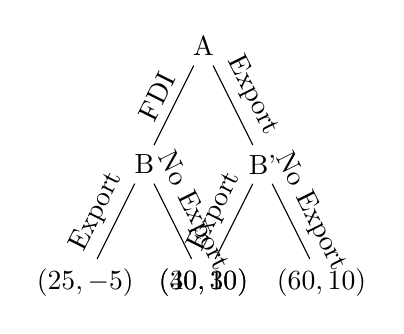
\begin{tikzpicture}[sloped]               
                \node {A}
                        child {                                
                                node {B}
                                        child {                
						node {$(25,-5)$} 
                                                edge from parent
                                                        node[above] {Export}
                                                }
                                        child {                 
                                                node {$(40,10)$} 
                                                edge from parent
                                                        node[above] {No Export}
                                                }
                                                edge from parent
                                                        node[above] {FDI}
                                }
                        child {                                
                                node {B'}
                                        child {                 
                                                node {$(30,30)$} 
                                                edge from parent
                                                        node[above] {Export}
                                                }
                                        child {                 
                                                node {$(60,10)$}
                                                edge from parent
                                                        node[above] {No Export}
                                                }
                                                edge from parent
                                                        node[above] {Export}
                                };
        \end{tikzpicture}

	\begin{itemize}
	\setlength\itemsep{0cm}
		\item In \textit{Normal Form}, (Export, Export) is the \textit{Dominant Strategy}, but there are more options:
		\begin{itemize}
			\item (Export, Export')
			\item (Export, No Export')
			\item (No Export, Export')
			\item (No Export, No Export')
		\end{itemize}
		\item If A plays FDI, will B ever export?
		\begin{itemize}
			\item (No Export, Export') allows \textit{Incredible Threats} to be made
		\end{itemize}
	\end{itemize}

		\subsubsection{Backwards Induction}

	\begin{itemize}
	\setlength\itemsep{0cm}
		\item A process used to avoid \textit{Incredible Threats}
		\item If A assumes B is rational, they expect B to play $(40,10)$ on FDI and $(30,30)$ on Export
		\item \textit{Credible Threats}:
		\begin{itemize}
			\item Only on FDI as they could lower their payoff to punish A
			\item $(25,-5)$
		\end{itemize}
	\end{itemize}

	\begin{enumerate}
	\itemsep\setlength{0cm}
		\item Start on that last stage of the game
		\item Break down into two of A's options
		\item Select these two \textit{Subgame Nash Equilibria} for B on each A arm
		\begin{itemize}
			\item (No Export, Export') are the best for B here
		\end{itemize}
		\item A now has a choice
		\begin{itemize}
			\item FDI would be followed by B's  No Export $(40,10)$ [$>(25,-5)$]
			\item Export would be followed by B's Export' $(30,30)$ [$<(60,10)$]
			\item A plays FDI
		\end{itemize}
		\item \textit{Nash Equilibrium} is made clear
		\begin{itemize}
			\item \{FDI,(Not Export, Export')\}
		\end{itemize}
	\end{enumerate}

		\subsubsection{Order Advantages}

	\begin{itemize}
	\setlength\itemsep{0cm}
		\item \textit{Commitment} in first mover vs. \textit{Flexibility} in follower
		\begin{itemize}
			\item Commitment has greater value in simultaneous games 
			\item Flexibility has greater value in sequential games
		\end{itemize}
		\item Recall that in simultaneous games there’s a first mover advantage
		\item \textit{First Mover Advantage} (Simultaneous):
		\begin{itemize}
			\item \begin{center}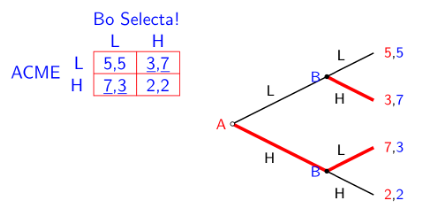
\includegraphics[width=6cm,height=3cm]{EC315-IMG/2.png}\end{center}
			\item B maximises on both moves and A maximises on its one move
			\item A lowers B’s payoff by choosing a more profitable option for them
		\end{itemize}
		\item \textit{Second Mover Advantage} (Sequential):
			\begin{itemize}                      
                        \item \begin{center}
\includegraphics[width=6.5cm,height=3cm]{EC315-IMG/3.png}\end{center}
                        \item M goes for overall highest payoff (6) by choosing move A
                        \item P has the option to choose one which greater benefits them and lowers M’s expected payoff
                \end{itemize}
	\end{itemize}

		\subsubsection{Manipulating Games}

	\begin{itemize}
	\setlength\itemsep{0cm}
		\item Take actions to manipulate a game? That is, guaranteeing the outcome
		\item \textit{Threats \& Promises}
		\begin{itemize}
			\item ``If you attack, I'll fight...''
			\item ``If you enter, I'll enter too; making it less profitable for you...''
			\item ``If you work hard, I'll work harder...''
			\item These lack credibility as they could be bluffs
		\end{itemize}
		\item \textit{Credibility}
		\begin{itemize}
			\item ``If you're late, I'll set off a bomb...'' (\textit{Incredible}; bluffing / not factual?)
			\item ``If you're late, the timed boomb will go off...'' (\textit{Credible}; more believable / factual)
			\item Changes first mover's thinking
		\end{itemize}
	\end{itemize}

		\subsubsection{Price Matching Guarantees}
	
	Standard \textit{Subgame Perfect Nash Equilibrium}:

	\begin{center}
		
\includegraphics[width=6cm,height=3cm]{EC315-IMG/4.png}
	\end{center}

	Offering a \textit{Price Match Guarantee}:

	\begin{center}
		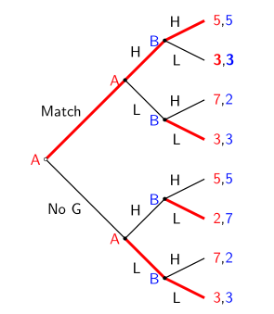
\includegraphics[width=4.5cm,height=6cm]{EC315-IMG/5.png}
	\end{center}

	\begin{itemize}
	\setlength\itemsep{0cm}
		\item Commitment to maintain high prices
		\item By committing to match low prices, A changes payoffs such that it’s not beneficial for B to undercut – as bigger payoff can’t be seen 
		\item Both firms end up paying high prices
		\item (Pricing) \textit{Prisoner’s Dilemma}
	\end{itemize}

	\newpage

	\subsection{Prisoner's Dilemma}

	\begin{itemize}
	\setlength\itemsep{0cm}
		\item \textit{Cooperate} or \textit{Defect}
		\item Mutual gain: \textit{Cooperate}
		\item Individual incentive: \textit{Defect}
		\item \textit{Pareto Efficienct Equilibrium}
		\item Recall: someone has a dominant strategy where there’s harm done to each other and they could be better off (Pareto Efficient). Self-interest doesn’t pay off. But, games can be repeated (e.g. price re-setting), e.g. lower price than opponent now (get more custom volume), makes opponent less-off (also poor for aggregate prices), firms may form a passive collusion where they both think opponents will set low so they both set high
		\item Both players have dominant strategy to defect but they could have a better result when the both cooperate. Hence, when choosing best interest, harm is done to the opponent when choosing to Defect for own interest, the opponent may choose to Cooperate so have a worse outcome
	\end{itemize}

	\begin{center}
		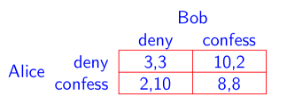
\includegraphics[width=5cm,height=2cm]{EC315-IMG/6.png}
	\end{center}

	Example:

	\begin{enumerate}
	\setlength\itemsep{0cm}
		\item (8,8) is Pareto Inefficient equilibrium as it is reached by both aiming for low by confessing. Could be made better off by both acting for mutual gain (3,3)
		\item Pricing – non-brand loyal market, flow freely between

		\item Team Work – (work vs shirk) shirk leads to more payoff as still full marks but no work done but if the other does all the work, they will get full marks but payoff will reduce due to workload
		\item Clean vs Dope – (risk based) best self-interest response is to dope as highest possible payoff but the equilibrium they both do it is less than the payoff if they both don’t
		\item Market Share – studying marketing is a waste of time. Market is a pie, we compete over our share. Ads try to [1] inform and [2] predatory (winning market share). Start: 50/50, engage in ads to win market share. I spend money, I get some in return but you won’t gain much more market share. The opponents do this to keep up. Each keep catching back up to 50\% each but both are still wasting millions on marketing. Market share isn’t changing proportionately but you’re still spending money
	\end{enumerate}

	\begin{center}
		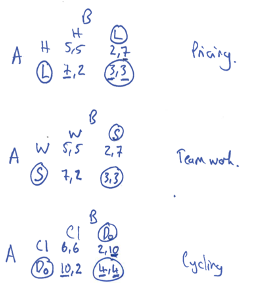
\includegraphics[width=3.5cm,height=4.5cm]{EC315-IMG/7.png}
	\end{center}

		\subsubsection{Externalities}

	\begin{itemize}
        \setlength\itemsep{0cm}
		\item \textit{Negative Externalities}: (own interest – doing too much) Cooperation reduces amount of work you do for the better (e.g. not over-fishing)
		\begin{itemize}
			\item Don’t see costs from defecting – too much harmful activity is done
		\end{itemize}
		\item \textit{Positive Externalities}: (own interest – doing too little) Cooperation says you should do more work (e.g. not doing no work in a project)
		\begin{itemize}
                        \item Don’t see costs benefits form cooperating – too little of a good activity is done
                \end{itemize}
		\item Example: Marginal Benefit vs. Marginal Cost – (1) extracting fish from the ocean makes it harder in the future (e.g. do less fishing to allow repopulation). (2) But you want more to sell now. (3) Self-interest makes it harder for others
	\end{itemize}

		\subsubsection{Rationalise Cooperation Resolutions}

	\begin{itemize}
        \setlength\itemsep{0cm}
		\item Resolutions to \textit{Prisoner's Dilemma}
		\item Meet-up (verbal agreement): let’s set high prices (incentive of deception however – you want him to set high prices and you want to set low)
		\item \textit{Threaten}: punishment of opponent doesn’t set high prices (lacking credibility as you ``will do it'' rather than it ``will be done (automatically etc.)'' – can fix credibility by using Mafia as they have more incentive to harm him)
		\item \textit{Reward}: offer a reward that overcomes the incentive to defect (still lacks credibility as it involves giving money – lowers your payoff. May not even believe you)
	\end{itemize}

		\subsubsection{Behavioural Resolution}
	
	\begin{itemize}
        \setlength\itemsep{0cm}
		\item \textit{External Norms of Behaviour}: Think back to litter e.g.: many people won’t actually litter even though it’s the most beneficial for you. It conflicts with the social norm
		\item \textit{Internal Norms of Behaviour}: Doing nice things for people who are nice to you (gain utility). Being bad to people but they are good to you (loss of utility). - you defect but if you care enough, you’ll maybe rationalise cooperation and change mind
	\end{itemize}

		\subsubsection{Price Matching Guarantee Resolution}

	\begin{itemize}                                         
        \setlength\itemsep{0cm}
		\item You may be undercut for opponent to gain market share from you at lower prices
		\item If you’re offered. PMG, you will simply match prices and keep customers ``he’s selling at that price, can you just sell me at that too''
		\item Opponent now doesn’t gain, just sells at lower price as no market gain
		\item Equilibrium of both pricing high – out of Prisoner’s Dilemma
	\end{itemize}

	\begin{center}
		
\includegraphics[width=4cm,height=4cm]{EC315-IMG/10.png}
	\end{center}

		\subsubsection{Dynamic Punishment Resolution}

	\begin{itemize}                                         
        \setlength\itemsep{0cm}
		\item When defecting, a player may believe they will be ‘punished’ in the future
		\item Can we achieve cooperation through fear of punishment?
		\begin{itemize}
			\item Credible: backed with fact
			\item Incredible: maybe won’t happen 
		\end{itemize}
		\item \textit{Finite Period} ($T$ Periods): defect in last period as no more time for retaliation
		\begin{itemize}
			\item Final period: mutual dominant strategy to defect as no future punishment 
			\item So: best to defect this period as well as you both will next
		\end{itemize}
		\item \textit{Infinite Period}: the game will continue [probability $p=1$] so retaliation 
		\begin{itemize}
			\item Always an opportunity to punish as there’s always another period
		\end{itemize}
		\item \textit{Impatient}: future worth less than present so defect (not caring for punishment)
		\item \textit{Patient}: care more for future gain by waiting and cooperating
	\end{itemize}
		
		\paragraph{Discounting}

	\begin{itemize}
	\setlength\itemsep{0cm}
		\item \pounds1 from \pounds1 today to \pounds1($1+r$) tomorrow; \pounds1 from \pounds1 tomorrow to \pounds$\frac{1}{(1+r)}$ today
		\item PV: $\frac{1}{(1+r)}$, $\frac{1}{(1+r)^2}$, ..., $\frac{1}{(1+r)^N}$; for discount rate $r$ and discount factor $\delta=\frac{1}{(1+r)^t}$
		\item Hence, \pounds$X$ in period $t$ is worth \pounds$X\frac{1}{(1+r)^t}$ today
		\item Hence, \pounds$X$ in period $t$ is worth \pounds$X\delta^t$ today
		\item $\delta$ close to 1: patient; $\delta$ close to 0: impatient
		\item CFs: $X_0,X_1,...,X_N$; PVs: $X_0+\delta X_1+\delta^2X_2+,...,+\delta^NX_N$
		\item Infinite: $1+\delta+\delta^2+\delta^3=\frac{1}{(1-\delta)}$
	\end{itemize}

	Example:

	\begin{center}
		
\includegraphics[width=6cm,height=2cm]{EC315-IMG/11.png}
	\end{center}

	\begin{center}
	\begin{tabular}{l|l}
		Payoff of 7 in perpetuity & Payoff of 10 today and 2 in perpetuity\\
		$7+7\delta+7\delta^2+...=7\frac{1}{1-\delta}$ & $10+2\delta+2\delta^2+...=10+2\delta\frac{1}{(1-\delta)}$
	\end{tabular}
	\end{center}

	\newpage

		\paragraph{Trigger Strategies: Grim Trigger}

	\begin{itemize}                
        \setlength\itemsep{0cm}
		\item Start by cooperating
		\item If opponent cooperated, cooperate
		\item If opponent defected, defected in perpetuity
	\end{itemize}

	\begin{enumerate}                                      
        \setlength\itemsep{0cm}
		\item \textit{Cooperate}:
		\begin{itemize}
			\item Opponent gets 600 forever $\rightarrow$ $600+600\delta+600\delta^2+...=\frac{600}{(1-\delta)}$
		\end{itemize}
		\item \textit{Defect}:
		\begin{itemize}                            
			\item Get 1000 now but 400 after $\rightarrow$ $1000+400\delta+400\delta^2+...=1000+\frac{400\delta}{(1-\delta)}$
                \end{itemize}
		\item Answer:
		\begin{itemize}                            
			\item $\frac{600}{(1-\delta)}\ge1000+\frac{400\delta}{(1-\delta)}\Leftrightarrow\delta\ge\frac{2}{3}(\Leftrightarrow\le\frac{1}{2})$ = 50\%
			\item \fbox{Hence, \textit{Grim Trigger} at $\delta>\frac{2}{3}$ so cooperate}
                \end{itemize}
	\end{enumerate}

		\paragraph{Trigger Strategies: Tit-for-Tat}

	\begin{itemize}
	\setlength\itemsep{0cm}                             
                \item Start by cooperating
		\item Play as the opponent played in the last round
		\item Cooperation followed by cooperation
		\item Defection frollowed by defection 
	\end{itemize}

	\begin{enumerate}                              
        \setlength\itemsep{0cm}                                   
                \item \textit{Defect} in perpetuity:                         
                \begin{itemize}                        
			\item Same as Grim Trigger: $\delta\ge\frac{2}{3}$
                \end{itemize}   
                \item \textit{Defect} once:
                \begin{itemize}       
			\item Get 400 now but loses 430 after $\rightarrow$ $400\le430\delta\Rightarrow\delta\ge\frac{40}{43}(\Rightarrow\le0.075)$ = 7.5\%
                \end{itemize}                              
                \item Answer:
                \begin{itemize}
                        \item \fbox{Hence, \textit{TFT} at $\delta>\frac{40}{43}$ so cooperate}
		\end{itemize}
        \end{enumerate}

	\fbox{If \textit{Grim} works: cooperation possible; If \textit{TFT} works: cooperation easy}

	\newpage

	\subsection{Games With Continuous Strategies}

	\begin{itemize}
	\setlength\itemsep{0cm}
		\item 
		\item 
		\item 
		\item 
		\begin{itemize}
			\item 
			\item 
			\item 
		\end{itemize}
		\item 
	\end{itemize}













\end{document}
